
%What do we want to test?

%Short term model:
%- the event specification; 
%        - new data: Bloomberg global
%        - requiring 2/3 SDs for the event rule
%        - mkt cap vs. value weighted. 

%Long term:
%- mkt cap vs. value weighted. 
%- event collection length


In this section I will examine the robustness of the results by altering the model variables or event requirements and re-estimate the results. The practice can lead to validation or invalidation along with advancement of the model specification.  

\subsection{Market model: event specification}
The requirement rule for event identification is based on the magnitude of events in relation to the average event for the individual firm. Thus, it seems plausible that an increase in the tightness of the requirement rule will lead to higher abnormal returns in absolute values.  
To address the issue I test whether the short term abnormal returns are sensitive to the methodology in specifying individual events. Specifically, I re-estimate the models with a requirement stating that the events should be more than, respectively, two and three standard deviations from the average event. A tighter event specification determine that fewer stocks will be included in the model as less events will be regarded as important. Consequently, the events included should be more negative or positive with a stricter rule. 

The results are reported in table \ref{tab: ST_significace}, which demonstrate that negative events continue to generate significant abnormal returns, while positive events does not. Due to the insignificance of positive events I will only present the plots of the negative abnormal returns. The graph of the positive events can be found in Appendix \ref{fig:ST_pos_sensi}. 


\begin{table}[ht]
\centering
\caption{AAR and CAAR (in \%) with new event rule (sd)} 
\begin{tabular}{lcccc}
  \hline  \hline
  & \multicolumn{2}{c}{Positive} &  \multicolumn{2}{c}{Negative}\\ \cline{2-3} \cline{4-5}  
  & 2 sd & 3 sd & 2 sd & 3 sd   \\   
 \hline
$AAR_{t=0}$ & $\underset{(0.875)}{0.051}$ & $\underset{(-0.278)}{-0.022}$  & $\underset{(-3.409)}{-0.522^{***}}$ & $\underset{(-3.024)}{-0.617^{***}}$ \\ 
$CAAR_{[-2;+2]}$  & $\underset{(0.283)}{0.031}$  & $\underset{(0.631)}{0.089}$  & $\underset{(-3.66)}{-0.714^{***}}$ & $\underset{(-2.648)}{-0.657^{***}}$ \\ 
$CAAR_{[-5;+5]}$  & $\underset{(1.197)}{0.195}$  & $\underset{(1.350)}{0.290}$  &$\underset{(-3.56)}{-0.902^{***}}$ & $\underset{(-2.782)}{-0.867^{***}}$ \\ 
$CAAR_{[-10;+10]}$  & $\underset{(-0.168)}{-0.035}$  & $\underset{(-0.062)}{-0.018}$  & $\underset{(-1.886)}{-0.652^{*}}$ & $\underset{(-1.686)}{-0.697^{*}}$ \\ 
   \hline \hline
   \multicolumn{5}{p{12cm}}{ \footnotesize $^* \; p\; <\; 0.1$, $ ^{**} \; p\; <\; 0.05$, $ ^{***} \; p\; <\; 0.01$  } \\
   \multicolumn{5}{p{13cm}}{\footnotesize The tables shows the CAAR associated with positive and negative news over an event window of 5, 10, and 21 days surrounding the event date along with the AAR on $t=0$. The models are split on the requirement rule for included events (2 or 3 sd).} \\
   \hline
\end{tabular}
\label{tab:ST_sensitivity}
\end{table}

The two new models based on negative events are compared to the original results (1 sd) in figure \ref{fig:ST_neg_sensitivity}. The AAR is presented in dotted lines and the CAAR in solid lines along with estimation requirements of 1 sd (red), 2 sd (green), and 3 sd (blue). For simplicity, I have skipped the confidence intervals along with the bars, which represented the relative amount of events. The similarities of the AAR and CAAR imply that the results are robust to changes in the event specification. While it is clear that enforcing a stronger sd requirement leads to lower AARs on the event date, no effect on the CAAR is present, visually, over the full event window. From table \ref{tab:ST_sensitivity}, the AAR on $t=0$ is, respectively, -0.52\% and -0.61\% for the 2 and 3 sd requirements compared to -0.37\% for the original 1 sd, meaning that the greatest instantaneous causal impact happens with a tight event rule. All are significant on the 1\% level. Intuitively, the investor reaction is more severe when events are identified as more important.  


\begin{figure} [h]
    \centering
    \caption{Negative news: $CAAR_{t=10}$}
    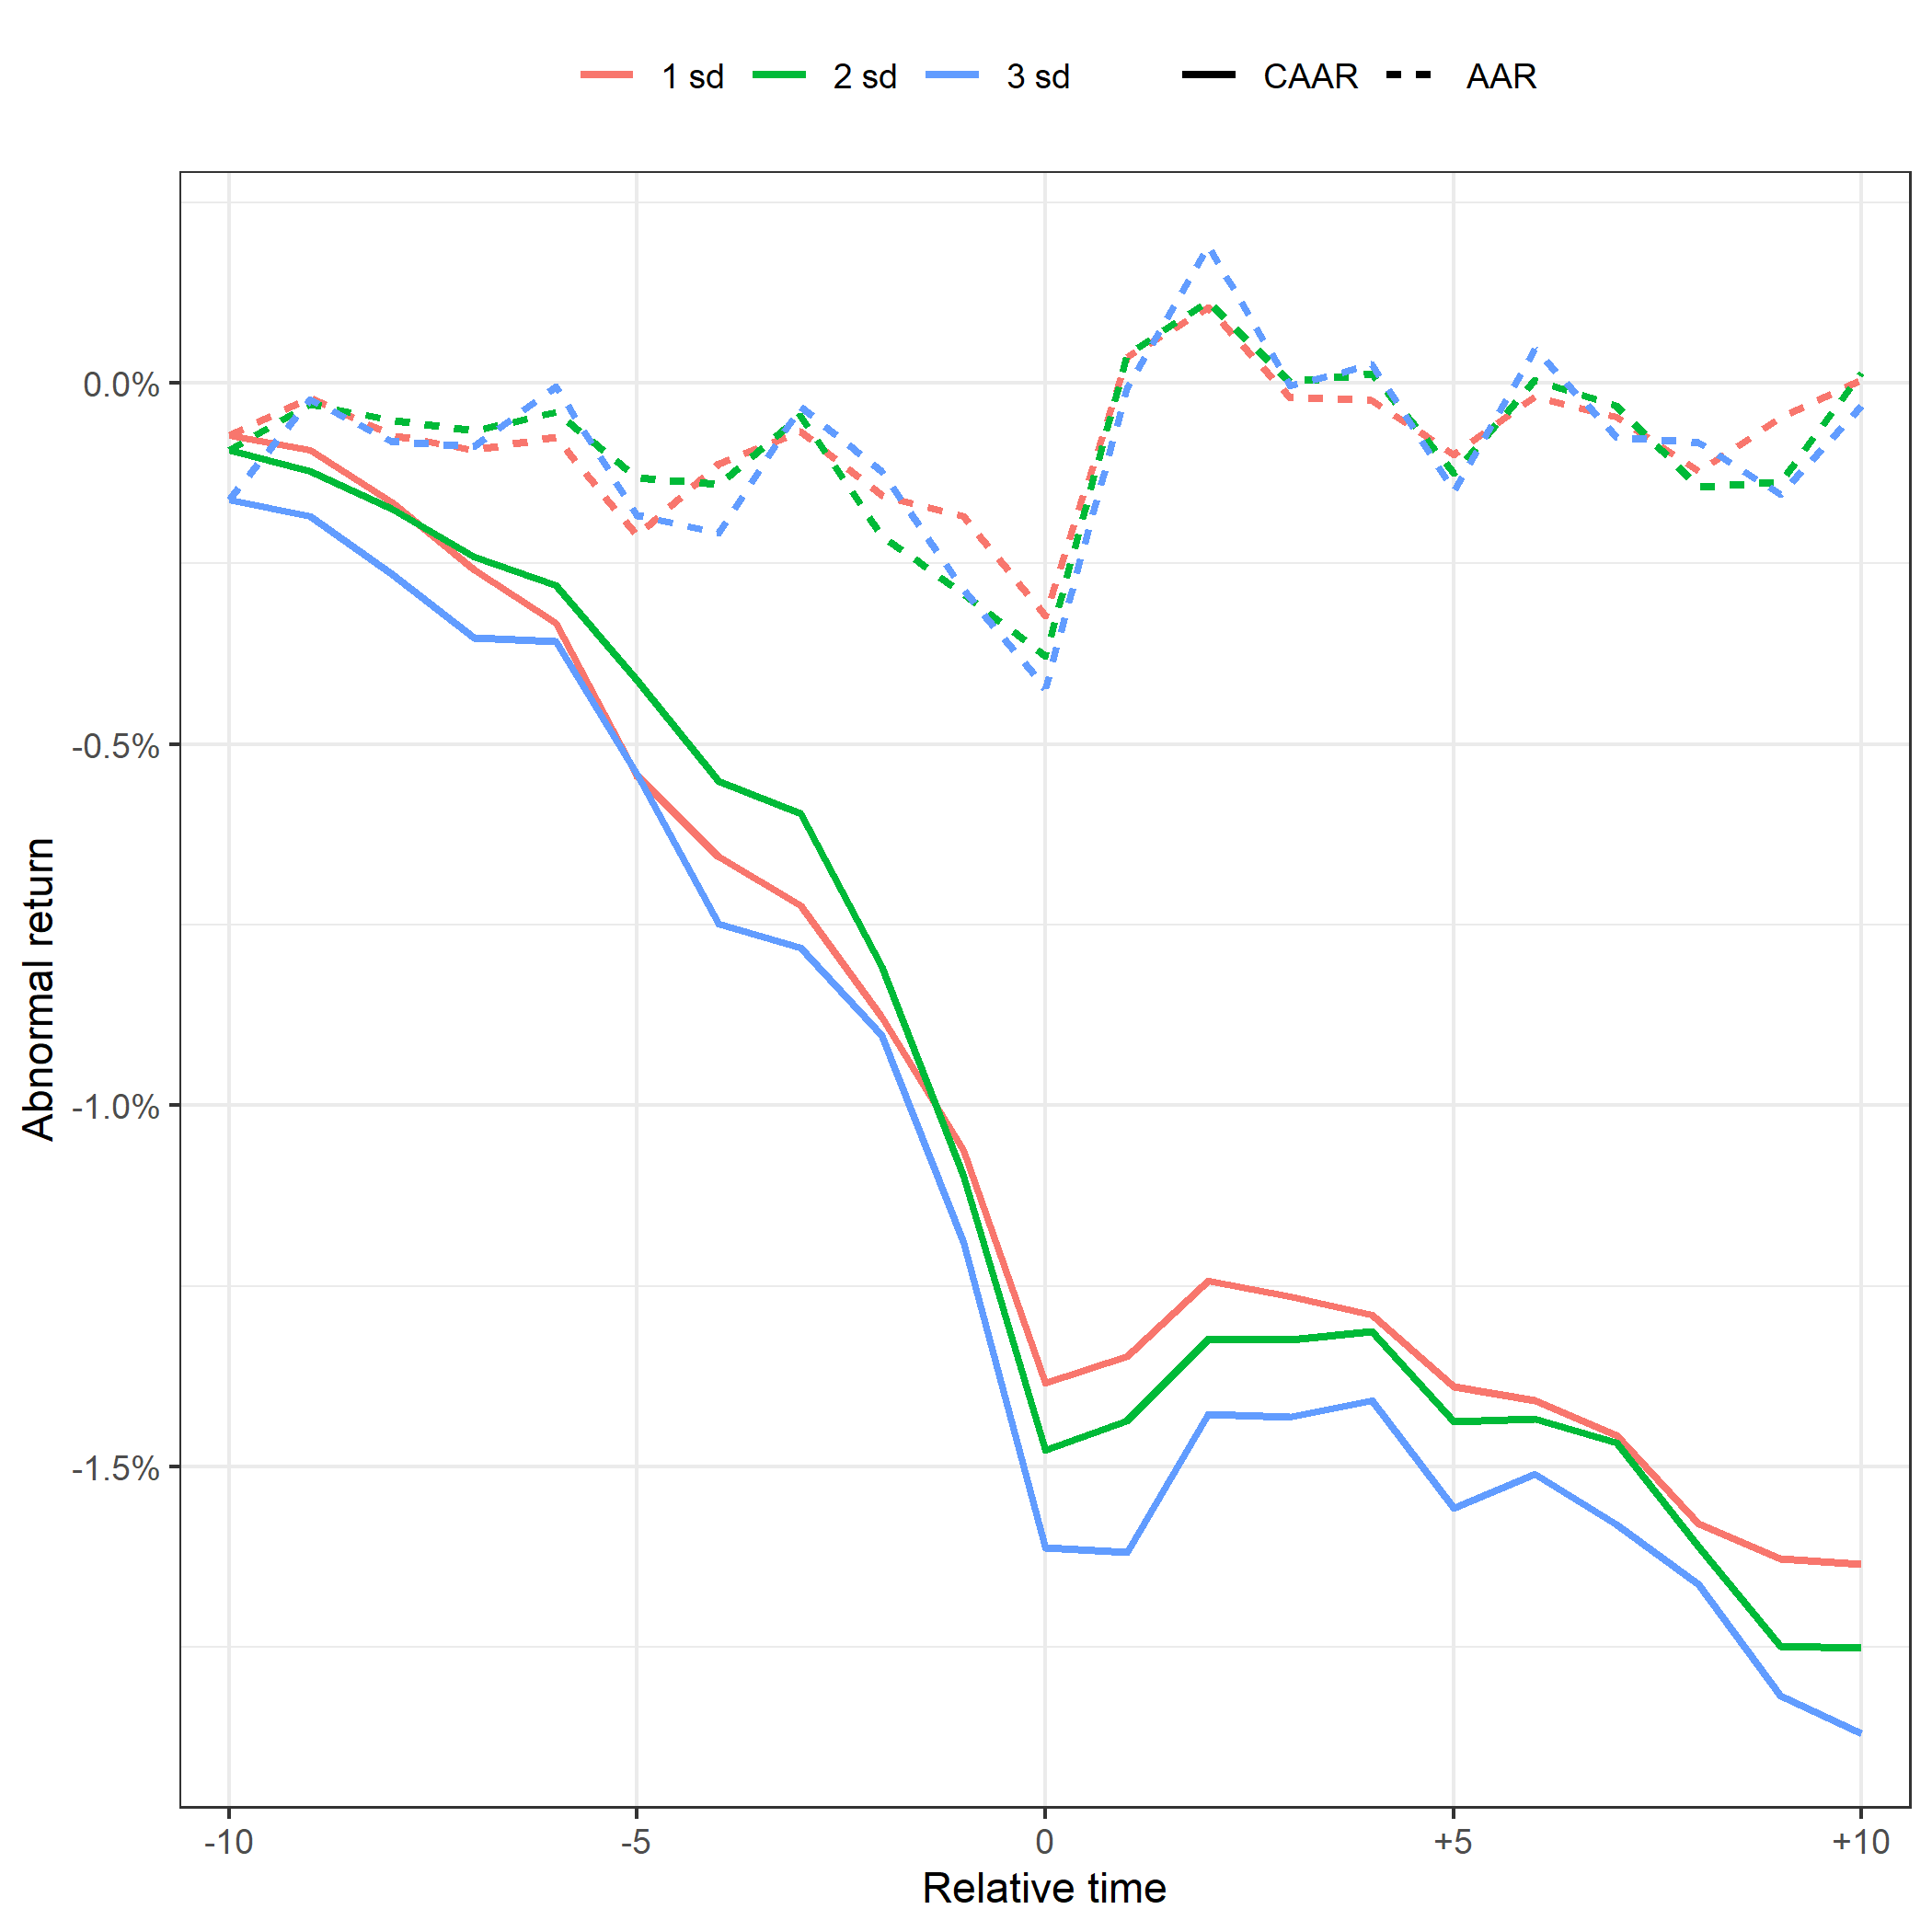
\includegraphics[scale=0.6]{Projekt/1.Figures analysis/ST_negative_sensitivity.png}
     \caption*{\footnotesize The figure illustrates the average abnormal return (AAR) and cumulative AAR (CAAR) around the event date (t = 0) of negative news. The lines (left axis) represent the average and the ribbons represent the 95th confidence intervals. The bars (right axis) represent the amount of events on a given day relative to t = 0. }
    \label{fig:ST_neg_sensitivity}
\end{figure} 


\subsection{Market model: value vs. equal weights}


\begin{figure} [H]
    \centering
    \caption{Negative news: $CAAR_{t=10}$}
    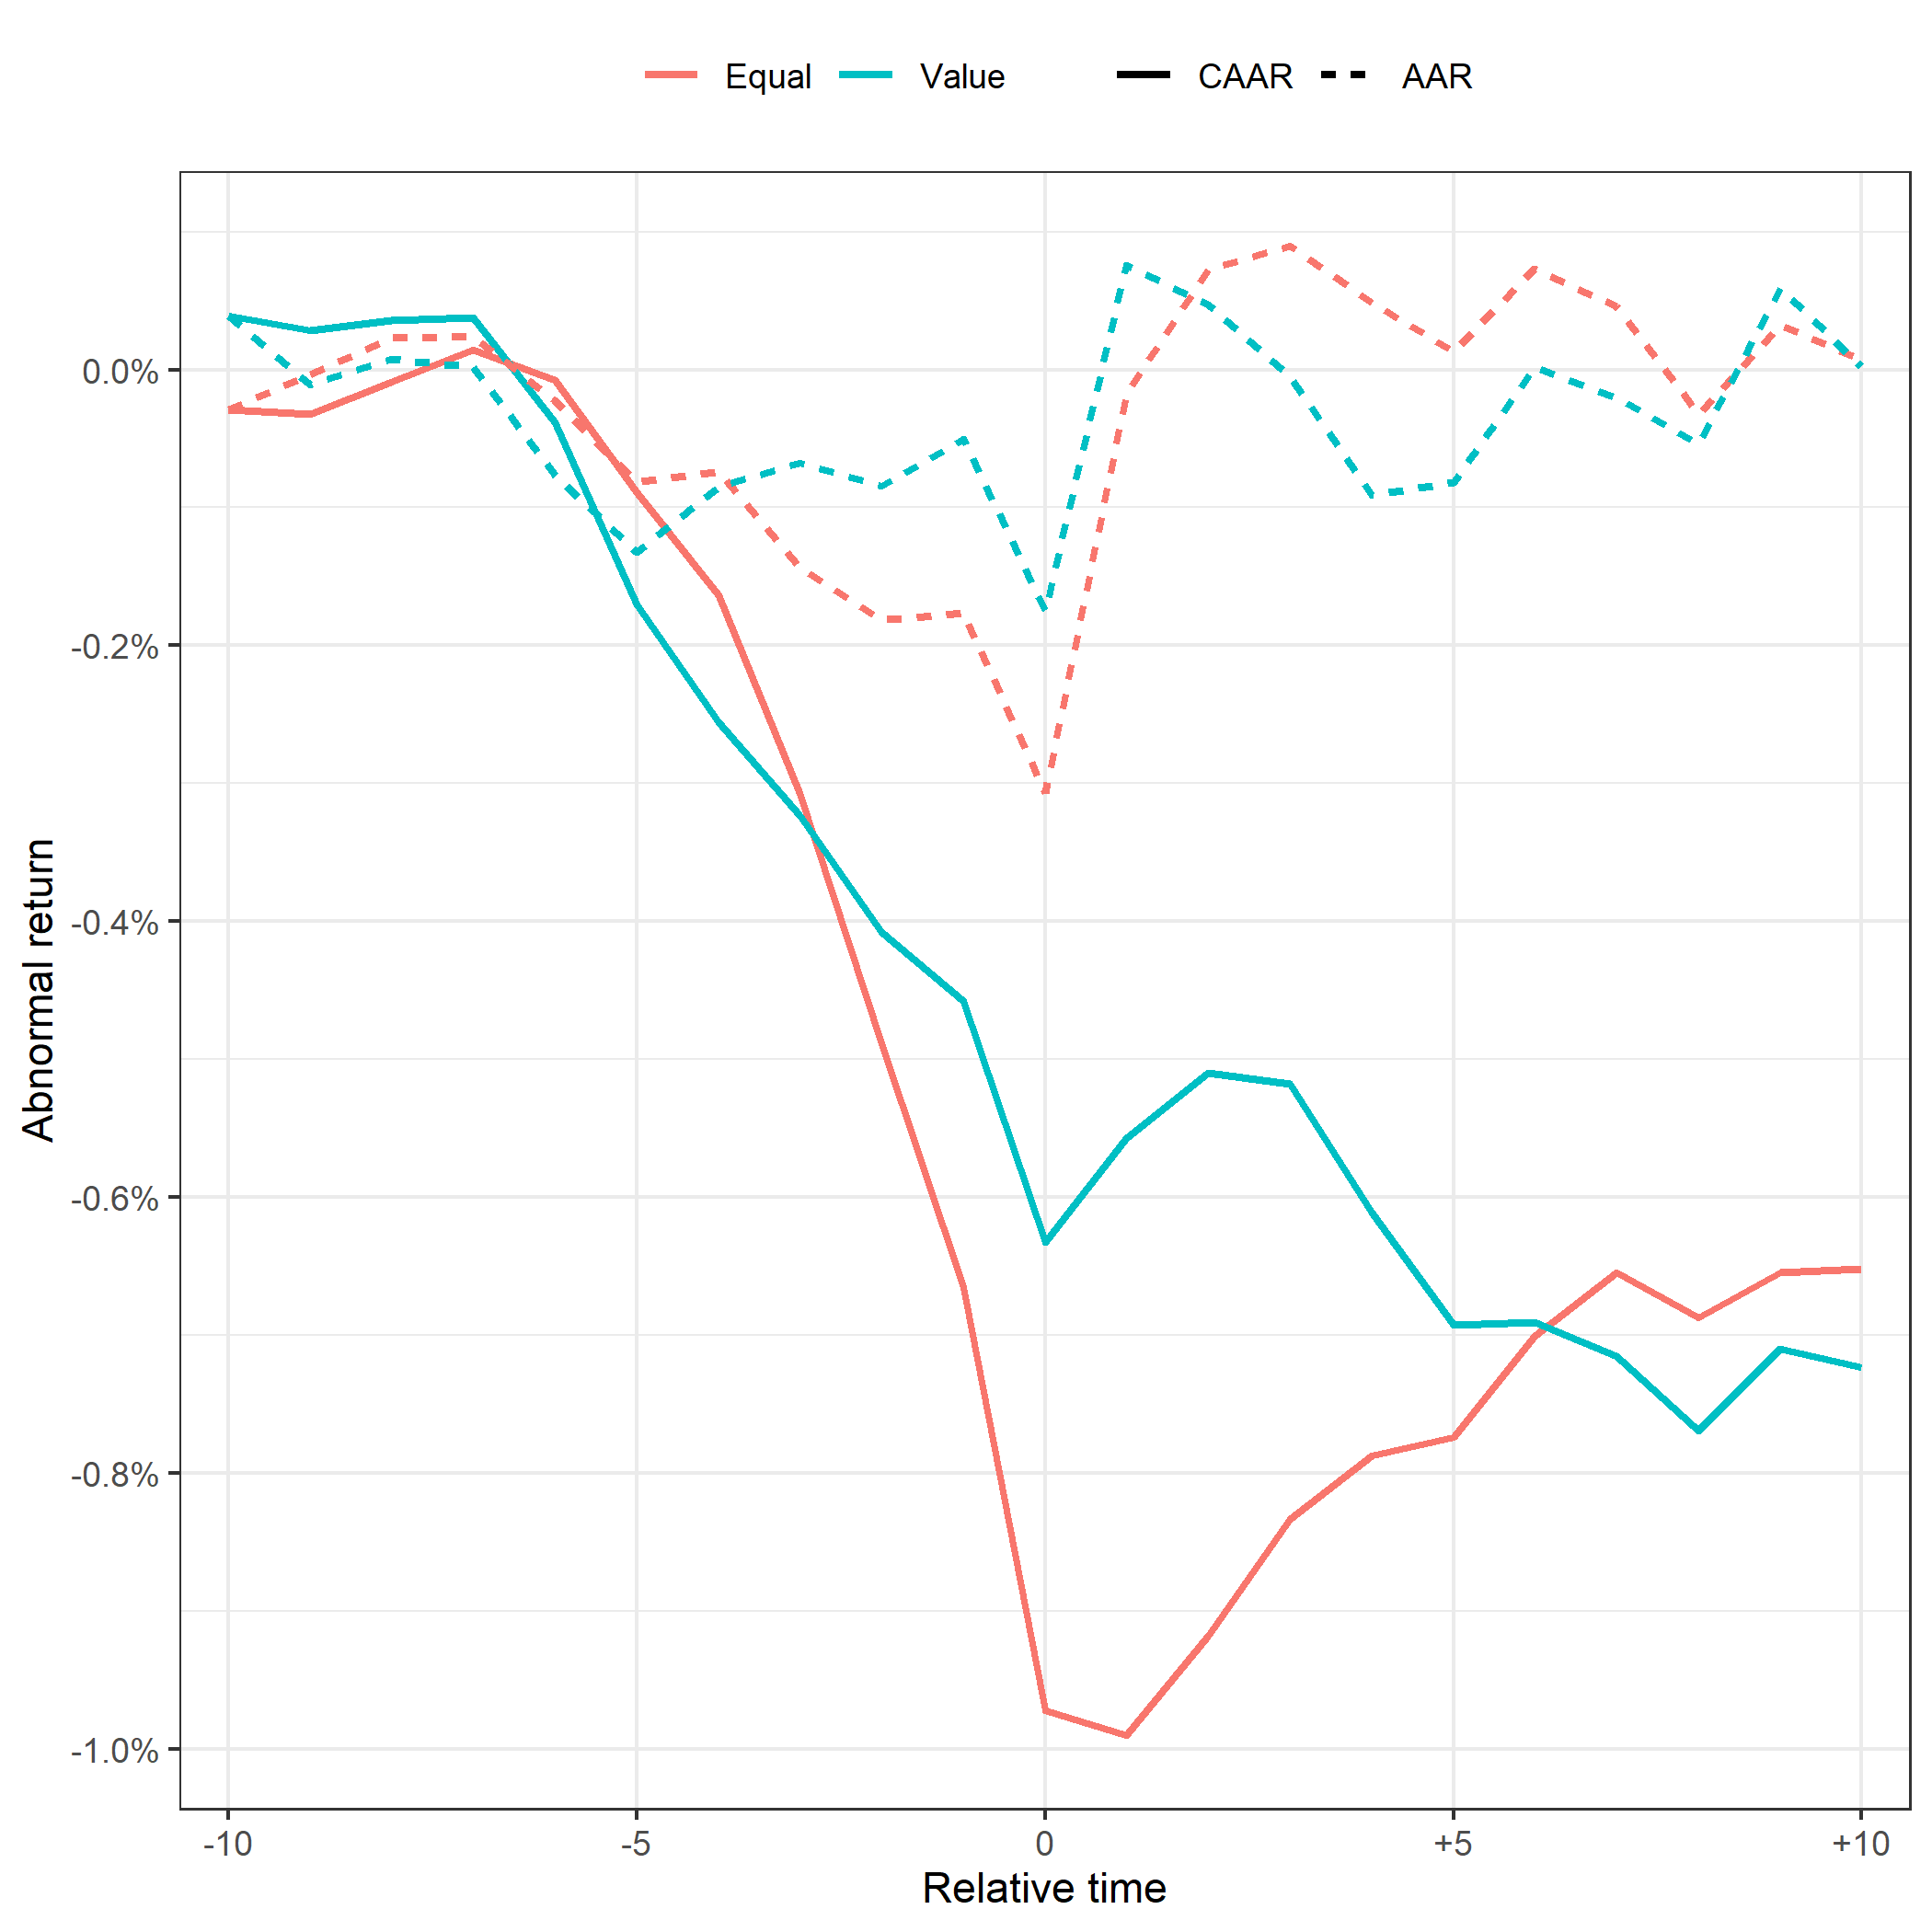
\includegraphics[scale=0.6]{Projekt/1.Figures analysis/ST_negative_sensitivity_weight.png}
     \caption*{\footnotesize The figure illustrates the average abnormal return (AAR) and cumulative AAR (CAAR) around the event date (t = 0) of negative news. The lines (left axis) represent the average and the ribbons represent the 95th confidence intervals. The bars (right axis) represent the amount of events on a given day relative to t = 0. }
    \label{fig:ST_neg_sensitivity_weight}
\end{figure} 

\subsection{Calendar Time Portfolio: }